\section{Results}
We confirmed that the level of experienced presence impacted spatial exploration behavior in VR. Interestingly the effect was similar across different mazes with a pattern of increasing presence associated with staying longer in the center of the maze and spending more time in segments \textit{presumably} critical for navigational success, i.e. corners. To emphasize the importance of considering individual differences when designing room-scale VR for a broad public, we carved out significant individual characteristics predicting the level of experienced presence, potentially of use for directing future design decisions.

\begin{figure}[h]
\centering
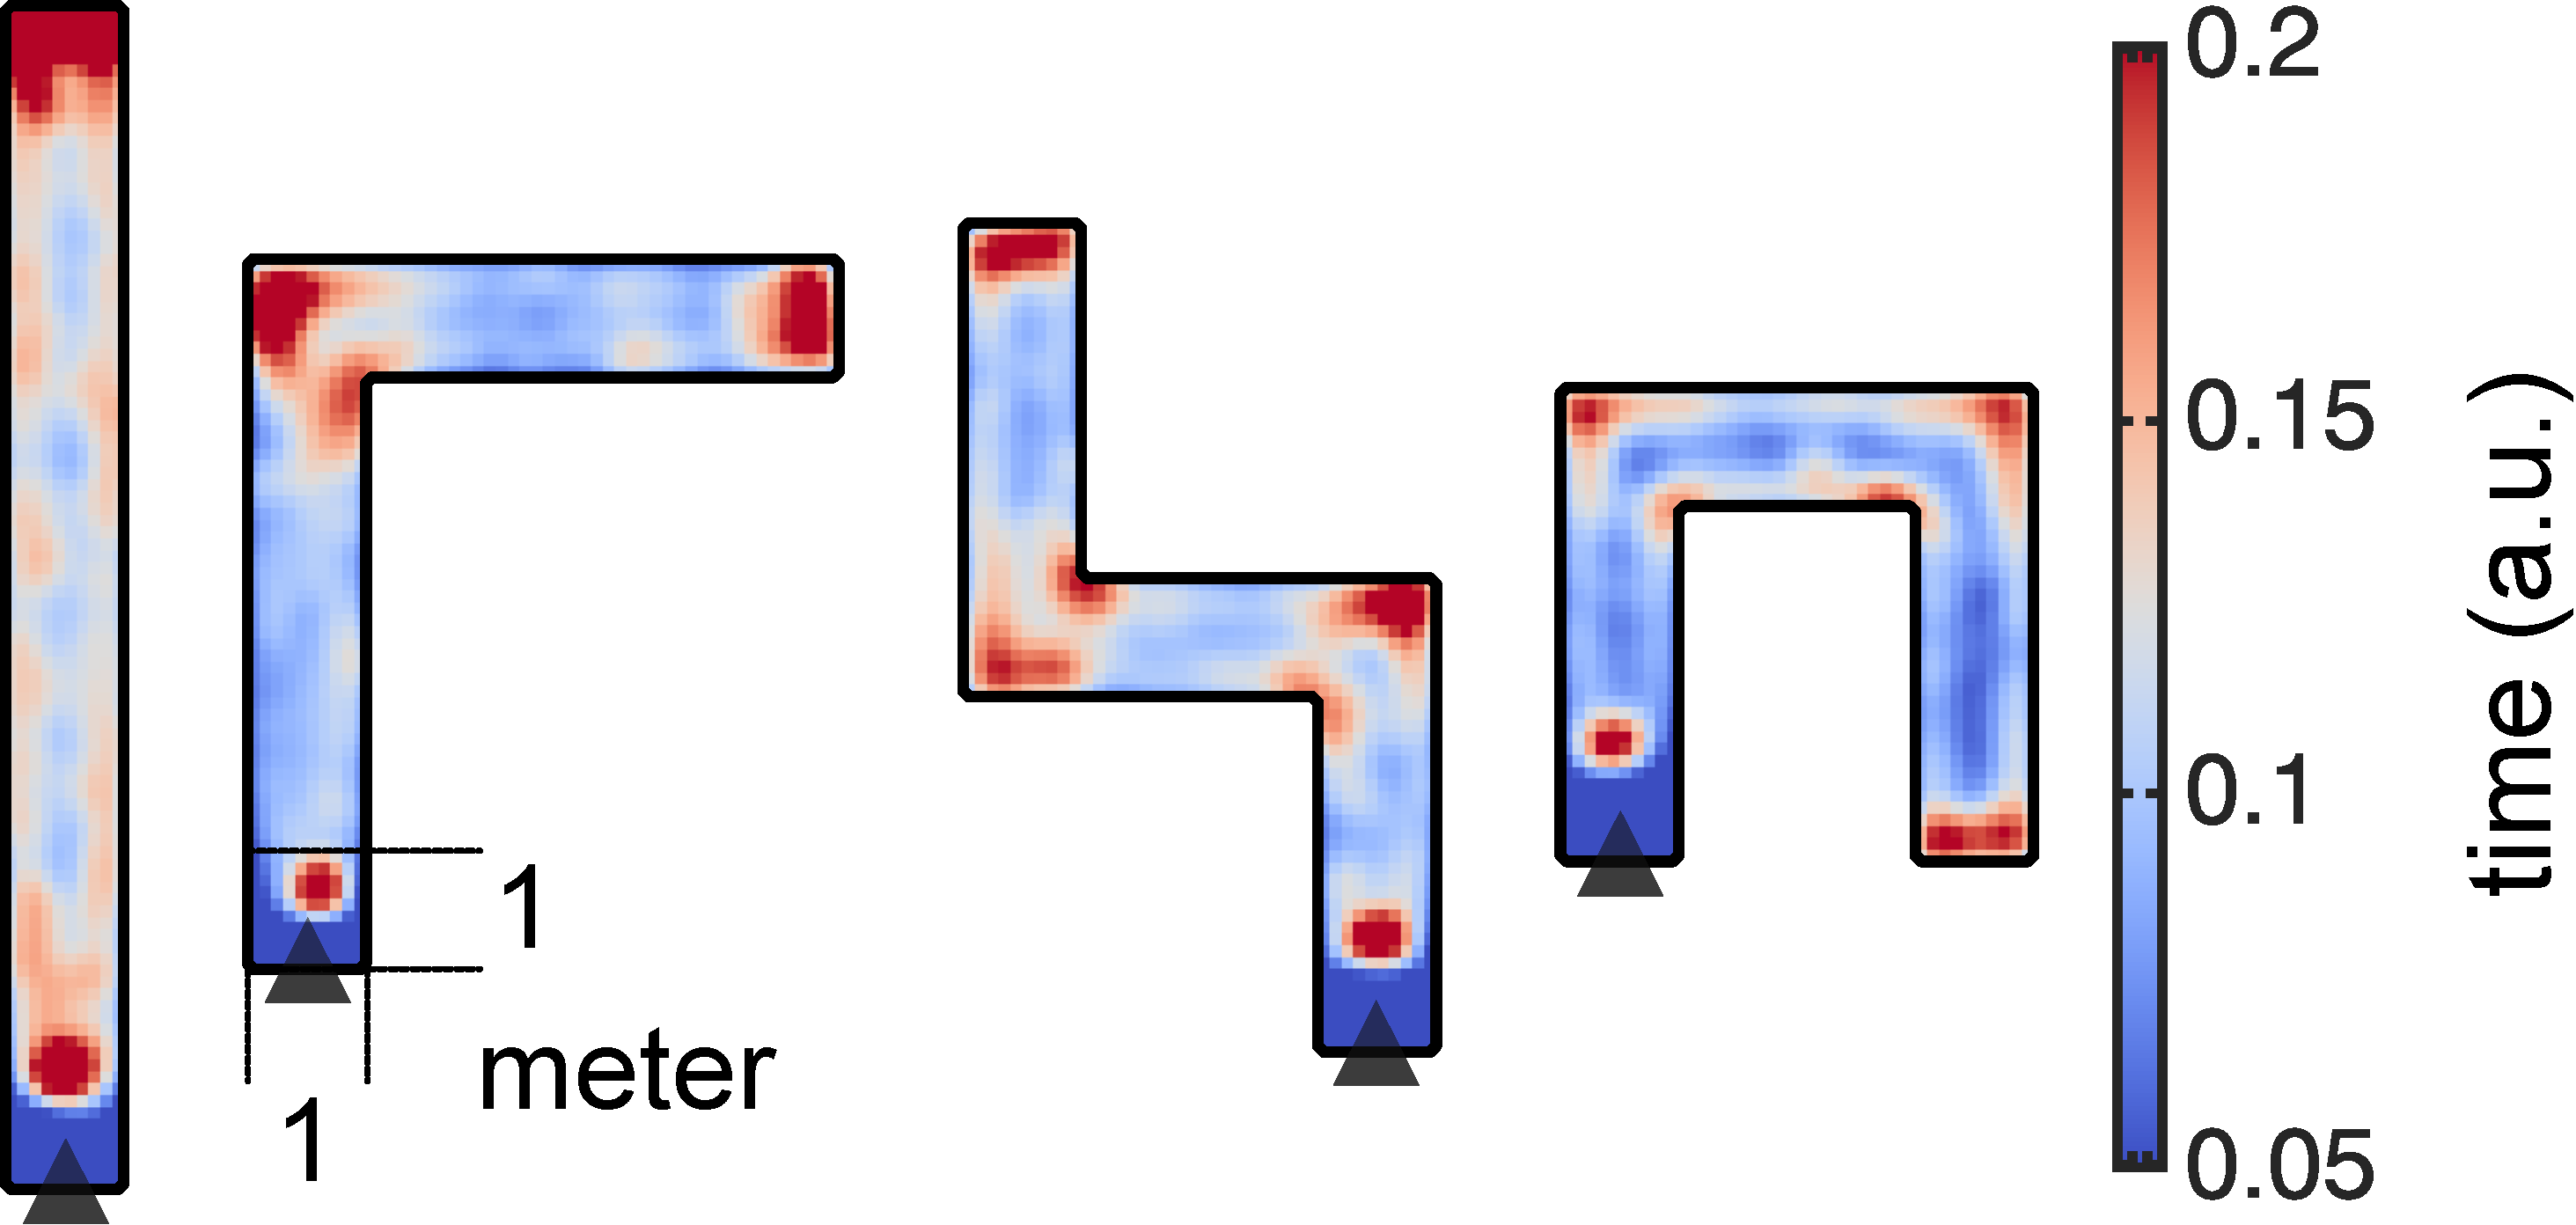
\includegraphics[width=\linewidth]{figures/head_loc_mean.pdf}
% \vspace{6pt}
\caption{Time spent at each location (grand-average) in each of the four mazes: `I', `L', `Z' and `U'. The whole lab space covered roughly 12 by 8 meters in size. Mazes are constructed of ten 1x1 meter squares. Warmer colors, i.e. red, indicate a longer time spent at that location. Green triangles indicate participants starting position.}
% \Description{Time spent at each location (grand-average) in each of the four mazes `I', `L', `Z' and `U' during exploration.}
\label{head_loc_mean}
\end{figure}